\documentclass{article}

\usepackage{booktabs} % for better table formatting
\usepackage{siunitx} % for aligning table columns by decimal point
\usepackage{graphicx}

\begin{document}

\title{\vspace{-3cm}CSCI 4320 Assignment 3 Report}
\author{Zhiqi Wang wangz56@rpi.edu}
\date{\today}
\maketitle

After implementing the $\texttt{MPI\_P2P\_Reduce}$ function, I ran it with different number
of ranks on AiMOS and compared the results with the $\texttt{MPI\_Reduce}$ function.

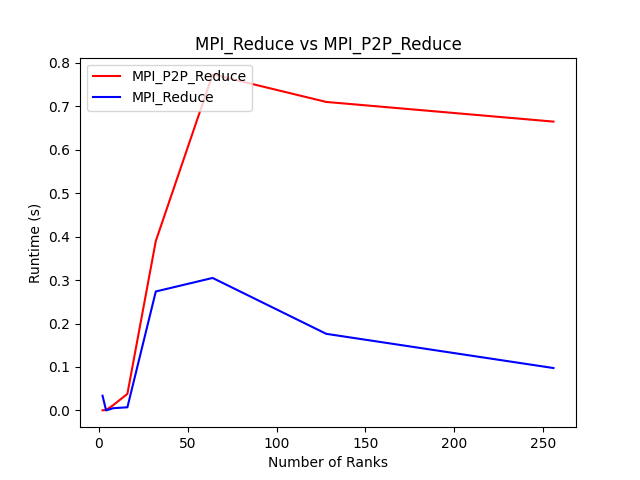
\includegraphics[width=\textwidth]{p2p-runtime.png}

Generally, while as the number of ranks increases from 2
ranks to 32 ranks, both function slows down. This could be due to the the over head of 
sending/receiving takes longer for more ranks. Then there's a slight speed up
for both function starting at 64 ranks, which we starting to use more than one node. 
This is suprising since we are using more than one node, which should create more 
overhead which would slow down the program (under the assumption that communication
across nodes is slower than within nodes). However, this is not the case. 
This could be due to the fact that as the number of ranks increases, the size of the 
data we are sending is decreasing. But this is not convincing since the size of the data
don't change much since the data type is fixed($\texttt{LONG\_LONG\_INT}$). In conclusion, 
I can't explain why there's a slight speed up for both function starting at 64 ranks. But 
what makes sense is that the $\texttt{MPI\_P2P\_Reduce}$ 's speed up is not as significant
as the $\texttt{MPI\_Reduce}$ 's speed up, since it requires more rounds of sending/receiving.


The $\texttt{MPI\_P2P\_Reduce}$ function is slower than the $\texttt{MPI\_Reduce}$ function
for all number of rank configurations. 
This is because the $\texttt{MPI\_P2P\_Reduce}$ function
need to receive/send messages for $\log_2 (\text{number of ranks})$ times while the
$\texttt{MPI\_Reduce}$ function only need to send/receive messages for one time.
We can see that as the number of ranks increases, the $\texttt{MPI\_P2P\_Reduce}$ function
takes more and more time since there's more rounds of sending/receiving messages and the 
overhead of each round is not negligible. 

\end{document}